\documentclass[12pt]{article}
\usepackage[utf8]{inputenc}
\usepackage{amsmath}
\usepackage{amssymb}
\usepackage{titlesec}
\usepackage{listings}
\usepackage{xcolor}
\usepackage{hyperref}
\usepackage{graphicx}
\usepackage{booktabs}

\titleformat{\subsection}
{\normalfont\normalsize\bfseries}{\thesubsection}{0.8em}{}

\lstdefinestyle{mystyle}{
    backgroundcolor=\color{white}, % Set background color
    basicstyle=\ttfamily\footnotesize, % Use a typewriter font
    commentstyle=\color{gray},     % Comment color
    keywordstyle=\color{blue},     % Keyword color
    numberstyle=\tiny\color{gray}, % Line number color
    stringstyle=\color{red},       % String color
    breaklines=true,               % Automatically break long lines
    frame=single,                  % Draw a frame around the code
    numbers=left,                  % Line numbers on the left
    numbersep=5pt,                 % Distance of line numbers from code
    showspaces=false,              % Don't show spaces
    showstringspaces=false,        % Don't show spaces in strings
    showtabs=false,                % Don't show tabs
    tabsize=4                      % Set default tab size
}

% Apply the custom style
\lstset{style=mystyle}

\usepackage{geometry}
\geometry{a4paper, margin=1in}

\usepackage[backend=biber, style=numeric, citestyle=numeric]{biblatex} % Load biblatex with the numeric style
\addbibresource{references.bib} % Specify the database of bibliographic references
\usepackage{hyperref} % For clickable links

\title{Sentiment Analysis Using Machine Learning}
\author{Davide Giuseppe Griffon}
\date{}

\titleformat{\paragraph}
{\normalfont\normalsize\bfseries}{\theparagraph}{1em}{}
\titlespacing*{\paragraph}
{0pt}{3.25ex plus 1ex minus .2ex}{1.5ex plus .2ex}

\begin{document}

\maketitle

\begin{abstract}
    This document serves as the report for the third task in the "Natural Language Processing" course completed by student Davide Giuseppe Griffon at Vilnius University as part of the Master's program in Data Science.
\end{abstract}

\tableofcontents

\newpage



\section{Dataset}
For this sentiment analysis project I used the IMDB Movie Reviews dataset. The dataset was loaded using the Python's \texttt{datasets} library, which provides a convenient interface for accessing various NLP datasets. The dataset contains binary sentiment labels: positive (1) and negative (0), representing the overall sentiment of each movie review.

The dataset consists of movie reviews from the Internet Movie Database (IMDB) and is structured as follows:
\begin{itemize}
   \item \textbf{Total Size}: 50,000 movie reviews
   \item \textbf{Split Distribution}:
       \begin{itemize}
           \item Training set: 25,000 reviews
           \item Testing set: 25,000 reviews
       \end{itemize}
   \item \textbf{Class Distribution}: The dataset is perfectly balanced, with:
       \begin{itemize}
           \item 50\% negative reviews (label 0)
           \item 50\% positive reviews (label 1)
       \end{itemize}
   \item \textbf{Review Length}: The average review length is 1,325 characters
\end{itemize}

The data was loaded and processed using a custom \texttt{load\_imdb\_dataset} function, which returns two separate pandas DataFrames: one for training and one for testing.

The balanced nature of the dataset is advantageous for training machine learning models because it eliminates the need for class weight adjustments or other imbalance-handling techniques that might otherwise be necessary. This is one of the main reasons I chose to use this particular dataset for this sentiment analysis task.


% -------------------------------------------------------------------------------------------------
% -------------------------------------------------------------------------------------------------
% -------------------------------------------------------------------------------------------------



\section{Preprocessing}
\paragraph{Data Loading and Sampling}
The initial step involves loading the IMDB dataset using the previously mentioned \texttt{load\_imdb\_dataset} function. For this project, I used a subset of 10,000 reviews (5,000 for training and 5,000 for testing) to optimize computational efficiency while maintaining result quality. This sampling approach allowed for faster preprocessing and training phases without compromising the effectiveness of the sentiment analysis.

\paragraph{Text Cleaning}
The \texttt{clean\_dataset} function implements several text cleaning steps:
\begin{itemize}
    \item Removal of missing values and empty cells to ensure data integrity.
    \item Elimination of HTML tags (such as \texttt{<br>}) found in the raw text through regex patterns.
    \item Removal of punctuation marks, retaining only alphanumeric characters through regex patterns.
    \item Conversion of all text to lowercase.
    \item Removal of stopwords using the \textit{spaCy} library.
\end{itemize}

\paragraph{Intermediate Data Storage}
To optimize the workflow and enable intermediate analysis, the preprocessing pipeline includes data persistence steps:

\begin{enumerate}
    \item The initially cleaned data (pre-lemmatization) is saved using \\ \texttt{save\_raw\_datasets\_to\_local} function, that stores the cleaned data in two separate CSV files: one for training and one for testing.
    \item This raw preprocessed data can be retrieved using \texttt{load\_local\_raw\_datasets} function.
\end{enumerate}
This intermediate storage allows for analysis of the data before and after lemmatization.

\paragraph{Lemmatization}
The final preprocessing step involves lemmatization and saves the fully preprocessed data to two new CSV files using the \texttt{save\_lemma\_datasets\_to\_local} function. To load the lemmatized data, the \texttt{load\_local\_lemma\_datasets} function can be used.
The steps involved in lemmatization are as follows:
\begin{itemize}
    \item Loads the raw preprocessed data using the \texttt{load\_local\_raw\_datasets} function.
    \item Applies \textit{spaCy}'s lemmatization to reduce words to their base form.
    \item Saves the fully preprocessed data to two separate CSV files: one for training and one for testing.
\end{itemize}

The separation of raw cleaning and lemmatization steps enables comparative analysis of their impact on the Word Cloud, as we'll see in the next section.


% -------------------------------------------------------------------------------------------------
% -------------------------------------------------------------------------------------------------
% -------------------------------------------------------------------------------------------------



\section{Word Cloud}
In order to visualize the most frequent words in the movie reviews and understand their distribution, I generated word clouds using the \textit{WordCloud} library. Word clouds provide an intuitive visualization where the size of each word is proportional to its frequency in the text corpus, making it easier to identify dominant themes and common expressions in the reviews.

\paragraph{Implementation}
The word cloud generation was implemented using a custom \texttt{generate\_word\_cloud} function that processes the text data and creates visualizations. This function was applied to both the raw preprocessed dataset and the lemmatized dataset to observe the effects of lemmatization on word frequencies:

\begin{itemize}
    \item For raw data: Applied after basic cleaning but before lemmatization
    \item For lemmatized data: Applied after all preprocessing steps, including lemmatization
\end{itemize}

\paragraph{Results Analysis}
\begin{figure}[h]
    \centering
    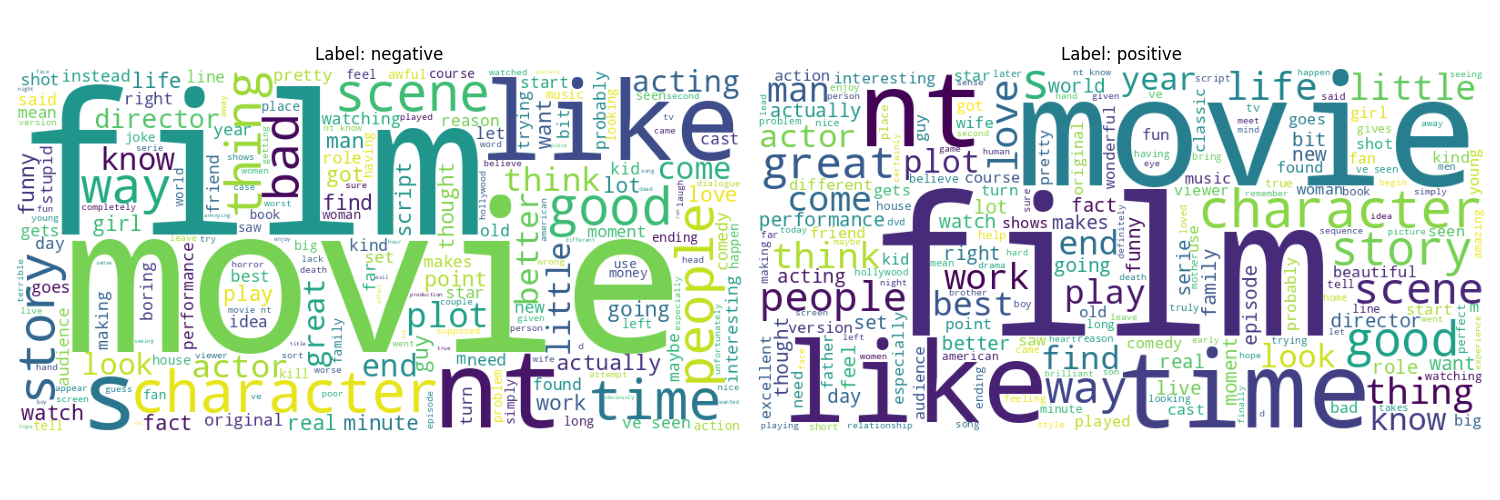
\includegraphics[width=0.8\textwidth]{raw_wordcloud.png}
    \caption{Word Cloud of Raw Preprocessed Reviews}
    \label{fig:raw_wordcloud}
\end{figure}

\begin{figure}[h]
    \centering
    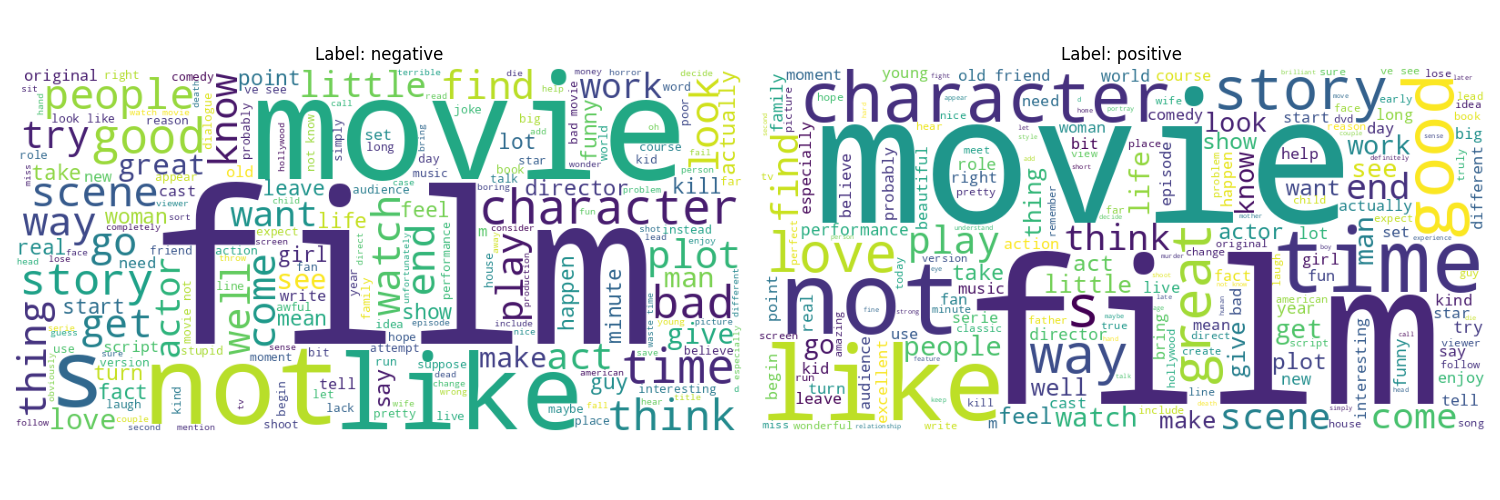
\includegraphics[width=0.8\textwidth]{lemma_wordcloud.png}
    \caption{Word Cloud of Lemmatized Reviews}
    \label{fig:lemma_wordcloud}
\end{figure}

Analysis of word frequencies reveals several interesting patterns:

\paragraph{General Observations}
\begin{itemize}
    \item \textbf{Domain-Specific Terms}: "movie" and "film" are consistently the most frequent words across both sentiment classes and preprocessing methods, indicating their role as domain identifiers rather than sentiment indicators.
    
    \item \textbf{Common Base Words}: Terms like "like", "time", "people", and "characters" appear frequently in both positive and negative reviews, suggesting they are neutral in sentiment.
\end{itemize}

\paragraph{Sentiment-Specific Patterns (after lemmatization)}
\begin{itemize}
    \item \textbf{Negative Reviews}:
        \begin{itemize}
            \item "bad" appears significantly more frequently (4,308 vs 2939 in positive reviews)
            \item Higher frequency of "not" (8,050 vs 5,419 in positive reviews)
            \item Focus on technical aspects: "plot", "acting", "scene"
        \end{itemize}
    
    \item \textbf{Positive Reviews}:
        \begin{itemize}
            \item Distinctive positive terms: "great" (2,775), "love" (2,259)
            \item "good" appears more frequently (4,347 vs 3,500 in negative reviews)
            \item More emphasis on emotional terms: "love", "great", "best"
        \end{itemize}
\end{itemize}

\paragraph{Impact of Lemmatization}
The lemmatization process had several notable effects:
\begin{itemize}
    \item \textbf{Word Consolidation - examples}: 
        \begin{itemize}
            \item "movie" and "movies" were consolidated, increasing the frequency from 9,493 to 11,188 in negative reviews
            \item "character" and "characters" were combined
            \item "watch", "watching", and "watched" were merged into "watch"
        \end{itemize}
    
    \item \textbf{Negation Handling}: The contraction "nt" was properly transformed to "not", making it more prominent in the frequency counts
    
    \item \textbf{Verb Forms}: Various forms of verbs were consolidated (e.g., "see"/"seen", "act"/"acting"), providing clearer frequency patterns
\end{itemize}

These findings suggest that while some words are strong indicators of sentiment ("bad", "great", "love"), many frequent terms are neutral and context-dependent. The lemmatization process helped clarify word usage patterns by consolidating different forms of the same word, potentially improving the accuracy of subsequent sentiment analysis steps.



% -------------------------------------------------------------------------------------------------
% -------------------------------------------------------------------------------------------------
% -------------------------------------------------------------------------------------------------



\section{Vectorization}
To convert the text data into a numerical format suitable for machine learning model training, I tried three distinct vectorization techniques: Word2Vec, Bag-of-Words (BoW), and Term Frequency-Inverse Document Frequency (TF-IDF).

\paragraph{Implementation Architecture}
I developed a dedicated \texttt{vectorization} module to handle all text vectorization processes. The module's core function \texttt{get\_vector\_datasets} provides a unified interface for accessing different vectorization methods:

\begin{lstlisting}[language=Python]
def get_vector_datasets(vectorization_type="tfidf"):
    vectorization_function = {
        "count": lambda: get_vector_datasets_bow("count"),
        "tfidf": lambda: get_vector_datasets_bow("tfidf"),
        "word2vec": get_vector_datasets_word2vec,
    }
    return vectorization_function[vectorization_type]()
\end{lstlisting}

\paragraph{Vectorization Methods}
The implementation leverages different libraries for each method:
\begin{itemize}
    \item \textbf{Word2Vec}: Implemented using the \textit{gensim} library
    \item \textbf{Bag-of-Words (BoW)}: Implemented using \textit{scikit-learn}'s \texttt{CountVectorizer}
    \item \textbf{TF-IDF}: Implemented using \textit{scikit-learn}'s \texttt{TfidfVectorizer}
\end{itemize}

\paragraph{Data Flow}
Each vectorization method follows a consistent workflow:
\begin{enumerate}
    \item Receives preprocessed training and testing datasets as separate pandas DataFrames
    \item Fits the vectorizer on the training data only to prevent data leakage
    \item Transforms both training and testing sets using the fitted vectorizer
    \item Returns vectorized versions of both datasets maintaining the original split
\end{enumerate}

In this way I could easy experiments with different vectorization techniques while maintaining consistent interfaces for the subsequent machine learning models. The default TF-IDF method was chosen based on preliminary experiments showing better performance with the movie review corpus.



% -------------------------------------------------------------------------------------------------
% -------------------------------------------------------------------------------------------------
% -------------------------------------------------------------------------------------------------


\section{Machine Learning Models}
Since in task 2 I already used a deep learning model, for this task I chose to try classical machine learning models. I experimented with four different models: Logistic Regression, Random Forest, Gradient Boosting and Support Vector Machine. I run all of them and compared their performance using the same vectorized data.

\paragraph{Implementation Details}
The code resides in the \texttt{models/classical\_models.py} file. All models were implemented using the \textit{scikit-learn} library. The function \texttt{classical\_models\_comparison} was used to run and compare models with the following configurations:

\begin{lstlisting}[language=Python]
models = {
    "Logistic Regression": LogisticRegression(
        random_state=RANDOM_STATE, max_iter=1000
    ),
    "Random Forest": RandomForestClassifier(
        n_estimators=100, random_state=RANDOM_STATE
    ),
    "Gradient Boosting": GradientBoostingClassifier(
        random_state=RANDOM_STATE
    ),
    "SVM": SVC(random_state=RANDOM_STATE),
}
\end{lstlisting}

Each model was trained and evaluated using the same vectorized dataset to ensure a fair comparison of their performance.



% -------------------------------------------------------------------------------------------------
% -------------------------------------------------------------------------------------------------
% -------------------------------------------------------------------------------------------------


\section{Results and Analysis}
I evaluated all models with each vectorization method, conducting a total of 4×3=12 experiments. The TF-IDF vectorization method demonstrated the best overall performance, and its results are presented below for each model.

In table \ref{tab:model-performance}, I present the performance metrics for each model using the TF-IDF vectorization method. The metrics include training accuracy, test accuracy, precision, and F1-score.

\begin{table}[h]
\centering
\caption{Model Performance Comparison}
\label{tab:model-performance}
\begin{tabular}{lcccc}
\toprule
\textbf{Model} & \textbf{Training Accuracy} & \textbf{Test Accuracy} & \textbf{Precision} & \textbf{F1-Score} \\
\midrule
Logistic Regression & 0.8902 & 0.8308 & 0.83 & 0.83 \\
Random Forest & 1.0000 & 0.8187 & 0.82 & 0.82 \\
Gradient Boosting & 0.8353 & 0.7989 & 0.80 & 0.80 \\
SVM & 0.9751 & 0.8400 & 0.84 & 0.84 \\
\bottomrule
\end{tabular}
\end{table}

\paragraph{Results Summary}
Among all tested models, SVM achieved the highest test accuracy (0.84), followed closely by Logistic Regression (0.83). Random Forest showed signs of overfitting with perfect training accuracy (1.0) but lower test accuracy (0.82). Gradient Boosting demonstrated the lowest performance with a test accuracy of 0.80. All models maintained balanced performance across classes, as evidenced by similar precision, recall, and F1-scores for both positive and negative reviews.



% -------------------------------------------------------------------------------------------------
% -------------------------------------------------------------------------------------------------
% -------------------------------------------------------------------------------------------------


\section{Conclusions}
The sentiment analysis task on IMDB movie reviews yielded several key findings:
\begin{itemize}
    \item TF-IDF vectorization consistently outperformed other vectorization methods
    \item SVM achieved the best performance with 84\% test accuracy
    \item All models maintained balanced performance between positive and negative classes
\end{itemize}

The results demonstrate that classical machine learning models can effectively perform sentiment analysis on movie reviews, despite modern deep learning models would probably achieve better results.

\newpage


% -------------------------------------------------------------------------------------------------
% -------------------------------------------------------------------------------------------------
% -------------------------------------------------------------------------------------------------



\section{Appendix - Code}

All the code is available in the GitHub repository \url{https://github.com/Griffosx/nlp} under the src/task\_3 folder.
For completeness, I include here the code for the main files used in this project.

File preprocessing.py
\begin{lstlisting}[language=Python]
from collections import Counter
import pandas as pd
from wordcloud import WordCloud
import matplotlib.pyplot as plt
from datasets import load_dataset
from task_3.constants import (
    nlp,
    POSITIVE_LABEL,
    TRAIN_RAW_DATA_PATH,
    TEST_RAW_DATA_PATH,
    TRAIN_LEMMA_DATA_PATH,
    TEST_LEMMA_DATA_PATH,
)

    
def load_imdb_dataset(
    num_samples=None, print_stats=False
) -> tuple[pd.DataFrame, pd.DataFrame]:
    """
    Load the IMDB movie reviews dataset for sentiment analysis.
    """
    # Load the dataset
    dataset = load_dataset("imdb")

    # Convert to pandas DataFrames
    train_df = pd.DataFrame(dataset["train"])
    test_df = pd.DataFrame(dataset["test"])

    # Sample if specified
    if num_samples:
        train_df = train_df.sample(min(num_samples, len(train_df)), random_state=42)
        test_df = test_df.sample(min(num_samples, len(test_df)), random_state=42)

    if print_stats:
        # Add some basic statistics
        print(f"Dataset Statistics:")
        print(f"Training samples: {len(train_df)}")
        print(f"Testing samples: {len(test_df)}")
        print(f"\nClass distribution in training:")
        print(train_df["label"].value_counts(normalize=True))
        # Calculate average review length
        train_df["review_length"] = train_df["text"].str.len()
        print(
            f"\nAverage review length: {train_df['review_length'].mean():.0f} characters"
        )

    return train_df, test_df


def clean_dataset(dataset: pd.DataFrame) -> pd.DataFrame:
    # Create a copy of the dataset
    cleaned_dataset = dataset.copy()

    # Remove missing values and empty cells
    cleaned_dataset = cleaned_dataset.dropna(subset=["text"])
    cleaned_dataset = cleaned_dataset[cleaned_dataset["text"].str.strip().astype(bool)]

    # Remove HTML tags
    cleaned_dataset["text"] = cleaned_dataset["text"].str.replace(
        r"<[^>]*>", "", regex=True
    )

    # Remove puntuation, leave only alphanumeric characters using regex
    cleaned_dataset["text"] = cleaned_dataset["text"].str.replace(
        r"[^\w\s]", "", regex=True
    )

    # Convert to lowercase
    cleaned_dataset["text"] = cleaned_dataset["text"].str.lower()

    # Remove stopwords using spaCy
    def clean_text(text):
        doc = nlp(text)
        # Keep only non-stopword tokens and strip spaces
        return " ".join(token.text.strip() for token in doc if not token.is_stop)

    cleaned_dataset["text"] = cleaned_dataset["text"].apply(clean_text)

    return cleaned_dataset


def load_and_clean_imdb_dataset(
    num_samples=None, print_stats=False
) -> tuple[pd.DataFrame, pd.DataFrame]:
    train_data, test_data = load_imdb_dataset(num_samples, print_stats)
    return clean_dataset(train_data), clean_dataset(test_data)


def save_raw_datasets_to_local(num_samples=None, print_stats=False):
    train_data, test_data = load_and_clean_imdb_dataset(num_samples, print_stats)
    train_data.to_csv(TRAIN_RAW_DATA_PATH, index=False)
    test_data.to_csv(TEST_RAW_DATA_PATH, index=False)


def load_local_raw_datasets() -> tuple[pd.DataFrame, pd.DataFrame]:
    train_data = pd.read_csv(TRAIN_RAW_DATA_PATH)
    test_data = pd.read_csv(TEST_RAW_DATA_PATH)
    return train_data, test_data


def save_lemma_datasets_to_local():
    train_data, test_data = load_local_raw_datasets()
    train_data["text"] = train_data["text"].apply(
        lambda x: " ".join([token.lemma_ for token in nlp(x)])
    )
    test_data["text"] = test_data["text"].apply(
        lambda x: " ".join([token.lemma_ for token in nlp(x)])
    )
    train_data.to_csv(TRAIN_LEMMA_DATA_PATH, index=False)
    test_data.to_csv(TEST_LEMMA_DATA_PATH, index=False)


def load_local_lemma_datasets() -> tuple[pd.DataFrame, pd.DataFrame]:
    train_data = pd.read_csv(TRAIN_LEMMA_DATA_PATH)
    test_data = pd.read_csv(TEST_LEMMA_DATA_PATH)
    return train_data, test_data


def generate_wordcloud(lemmatisation=True):
    """
    For each label in the dataset, generate and plot a wordcloud and print the top 20 most frequent words.
    """
    if lemmatisation:
        dataset, _ = load_local_lemma_datasets()
    else:
        dataset, _ = load_local_raw_datasets()

    # Get unique labels from the dataset
    unique_labels = dataset["label"].unique()

    # Create a figure with subplots for each label
    fig, axes = plt.subplots(1, len(unique_labels), figsize=(15, 5))

    for idx, label in enumerate(unique_labels):
        # Filter text for current label
        texts = dataset[dataset["label"] == label]["text"]

        text = " ".join(texts)

        # Generate word frequency distribution
        words = text.split()
        word_freq = Counter(words)

        # Get top 20 words and their frequencies
        top_20 = word_freq.most_common(20)

        # Print top 20 words for current label
        print(
            f"\nTop 20 most frequent words for {'positive' if label == POSITIVE_LABEL else 'negative'} reviews:"
        )
        print("{:<15} {:<10}".format("Word", "Frequency"))
        print("-" * 25)
        for word, freq in top_20:
            print("{:<15} {:<10}".format(word, freq))

        # Generate wordcloud
        wordcloud = WordCloud(
            width=800, height=400, background_color="white", stopwords=set()
        ).generate(text)

        # Plot wordcloud
        if len(unique_labels) > 1:
            axes[idx].imshow(wordcloud)
            axes[idx].axis("off")
            axes[idx].set_title(
                f"Label: {'positive' if label == POSITIVE_LABEL else 'negative'}"
            )
        else:
            axes.imshow(wordcloud)
            axes.axis("off")
            axes.set_title(
                f"Label: {'positive' if label == POSITIVE_LABEL else 'negative'}"
            )

    plt.tight_layout()
    plt.show()
    
\end{lstlisting}

File vectorization/bow.py
\begin{lstlisting}[language=Python]
from sklearn.feature_extraction.text import CountVectorizer, TfidfVectorizer
import pandas as pd
from task_3.preprocessing import load_local_lemma_datasets


def create_bow_datasets(
    train_dataset,
    test_dataset,
    vectorizer_type="count",
    max_features=1000,
    ngram_range=(1, 1),
):
    """
    Create BOW vectors using either CountVectorizer or TfidfVectorizer
    """
    # Choose vectorizer
    if vectorizer_type == "tfidf":
        vectorizer = TfidfVectorizer(
            max_features=max_features, ngram_range=ngram_range, min_df=2
        )  # Ignore terms that appear in less than 2 documents
    else:
        vectorizer = CountVectorizer(
            max_features=max_features, ngram_range=ngram_range, min_df=2
        )

    # Fit and transform training data
    X_train = vectorizer.fit_transform(train_dataset["text"])

    # Transform test data
    X_test = vectorizer.transform(test_dataset["text"])

    # Convert to DataFrames
    feature_names = vectorizer.get_feature_names_out()

    train_df = pd.DataFrame(X_train.toarray(), columns=feature_names)
    train_df["sentiment"] = train_dataset["label"]

    test_df = pd.DataFrame(X_test.toarray(), columns=feature_names)
    test_df["sentiment"] = test_dataset["label"]

    # Print some information about the vectorization
    print(f"Vocabulary size: {len(vectorizer.vocabulary_)}")
    print(f"Feature matrix shape: {X_train.shape}")
    print("\nMost common terms:")
    if vectorizer_type == "count":
        term_frequencies = X_train.sum(axis=0).A1
        top_terms = sorted(
            zip(vectorizer.get_feature_names_out(), term_frequencies),
            key=lambda x: x[1],
            reverse=True,
        )[:10]
        for term, freq in top_terms:
            print(f"{term}: {freq}")

    return train_df, test_df


def get_vector_datasets(vectorization_type="count"):
    train_dataset, test_dataset = load_local_lemma_datasets()

    train_dataset, test_dataset = create_bow_datasets(
        train_dataset, test_dataset, vectorization_type
    )

    return train_dataset, test_dataset
\end{lstlisting}

File models/classical\_models.py
\begin{lstlisting}[language=Python]
from sklearn.ensemble import RandomForestClassifier, GradientBoostingClassifier
from sklearn.svm import SVC
from sklearn.linear_model import LogisticRegression
from sklearn.metrics import accuracy_score, classification_report
from sklearn.preprocessing import StandardScaler
from task_3.vectorization import get_vector_datasets


RANDOM_STATE = 42


def classical_models_comparison():
    # Get data
    train_df, test_df = get_vector_datasets("word2vect")

    # Prepare features and labels
    X_train = train_df.drop("sentiment", axis=1).values
    y_train = train_df["sentiment"].values
    X_test = test_df.drop("sentiment", axis=1).values
    y_test = test_df["sentiment"].values

    # Scale features
    scaler = StandardScaler()
    X_train_scaled = scaler.fit_transform(X_train)
    X_test_scaled = scaler.transform(X_test)

    # Define models to try
    models = {
        "Logistic Regression": LogisticRegression(
            random_state=RANDOM_STATE, max_iter=1000
        ),
        "Random Forest": RandomForestClassifier(
            n_estimators=100, random_state=RANDOM_STATE
        ),
        "Gradient Boosting": GradientBoostingClassifier(random_state=RANDOM_STATE),
        "SVM": SVC(random_state=RANDOM_STATE),
    }

    # Try each model
    for name, model in models.items():
        print(f"\nTraining {name}...")
        model.fit(X_train_scaled, y_train)

        # Make predictions
        train_pred = model.predict(X_train_scaled)
        test_pred = model.predict(X_test_scaled)

        # Print results
        print(f"{name} Results:")
        print(f"Training Accuracy: {accuracy_score(y_train, train_pred):.4f}")
        print(f"Test Accuracy: {accuracy_score(y_test, test_pred):.4f}")
        print("\nDetailed Test Report:")
        print(classification_report(y_test, test_pred))

        # For Random Forest and Gradient Boosting, print feature importance
        if hasattr(model, "feature_importances_"):
            importances = model.feature_importances_
            top_features = sorted(
                zip(range(len(importances)), importances),
                key=lambda x: x[1],
                reverse=True,
            )[:10]
            print("\nTop 10 Most Important Features:")
            for idx, importance in top_features:
                print(f"Feature {idx}: {importance:.4f}")
\end{lstlisting}


\end{document}